

The domain is a spherical shell centered around the origin of the Cartesian 
axis system $(x,y,z)$. 
The inner radius is denoted by $R_1$ and the outer radius by $R_2$.
The Stokes equations are solved in the domain and the flow is assumed 
to be instantaneous, incompressible and isothermal.

The velocity in Cartesian coordinates is denoted by $\vec{v}=(v_x,v_y,v_z)$ and 
$\vec{v}=(v_r,v_\theta,v_\phi)$ in spherical coordinates. 
The equations to solve are then

\begin{eqnarray}
- \vec\nabla p + \vec\nabla \cdot (2 \eta \dot{\bm \varepsilon}(\vec v))  + \rho \vec{g} &=& 0 \\
\vec\nabla \cdot \vec{v} &=& 0
\end{eqnarray}
The domain has two boundaries: the inner boundary $r=R_1$ and the outer boundary at $r=R_2$.
Boundary conditions can be either no slip, free slip or open ('free surface').

The domain is filled with a fluid (the mantle 'm') of viscosity $\eta_m(\vec{r})$ 
and density $\rho_m(\vec{r})$.
A sphere ('s') of a different fluid or radius $R_s$ is placed at location $(0,0,z_s)$ with 
viscosity $\eta_s$ and density $\rho_s$. As such the setup is 
axisymmetric along the North-South poles line.
The gravity $\vec{g}=-g \vec{e}_r$ points towards the center of the shell\footnote{unless 
self gravitation is used}.

\begin{center}
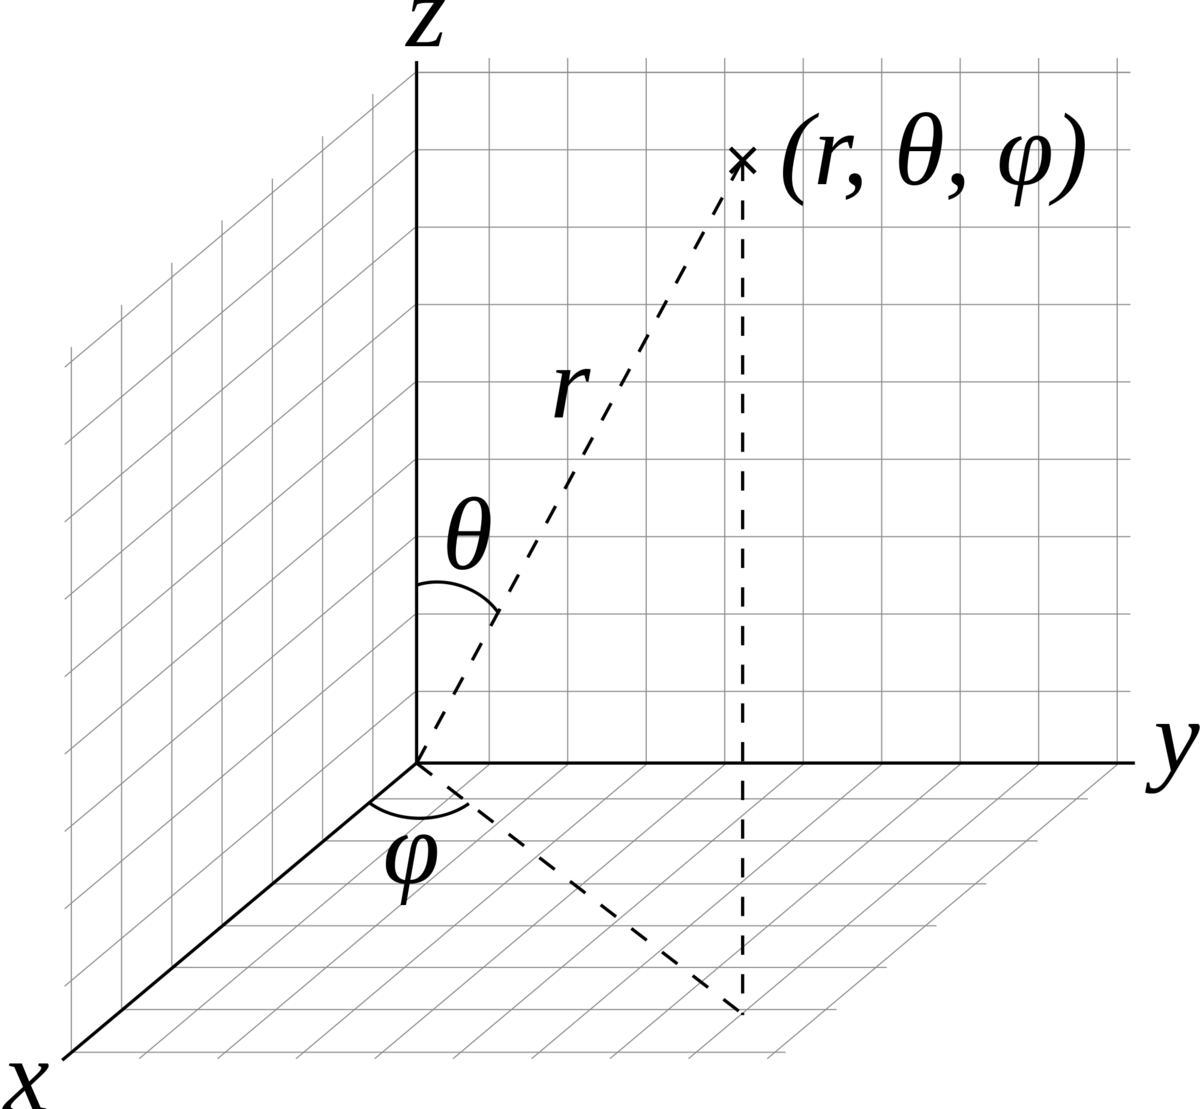
\includegraphics[width=6.5cm]{images/sphcoord}
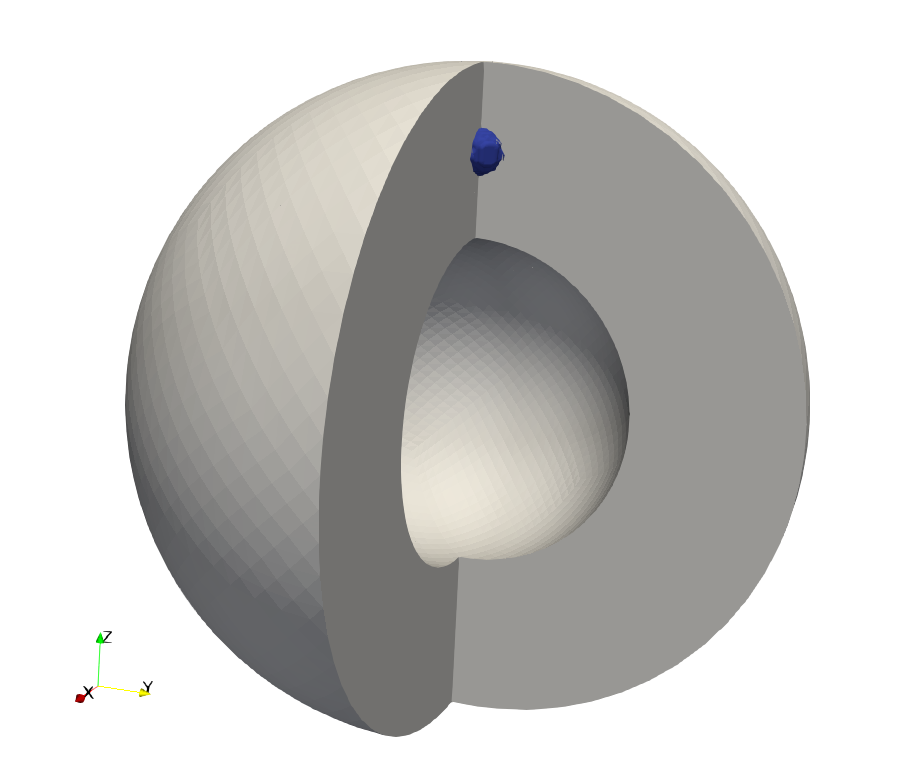
\includegraphics[width=8cm]{images/setup}
\end{center}

Models with free slip boundary conditions on both inner and outer surfaces have a rotational nullspace which needs to be removed. 

In such case the pressure also showcases a constant value nullspace which can be removed by ensuring that the average surface pressure is zero.
